\section{Compiladores}
Un compilador no es mas que un programa que basicamente, toma el codigo C 
y lo traduce a codigo de maquina. Existen varios para C, como ser GCC, Clang y el Compilador de Intel. Lo que vamos a hacer es compilar el codigo con Clang/GCC y ver si encontramos diferencias.Para comparar, se van a usar la version 4.8.4 de GCC y la 3.4 de Clang. 
Para realizar la comparacion, vamos a compilar el TP con GCC y luego con Clang.
Para empezar, vamos a comparar con optimizacion nula
Aqui el grafico de GCC

\begin{figure}[H]
    \centering
    \begin{floatrow}
      \ffigbox[\FBwidth]{\caption{Filtros con GCC -O0}}{%
        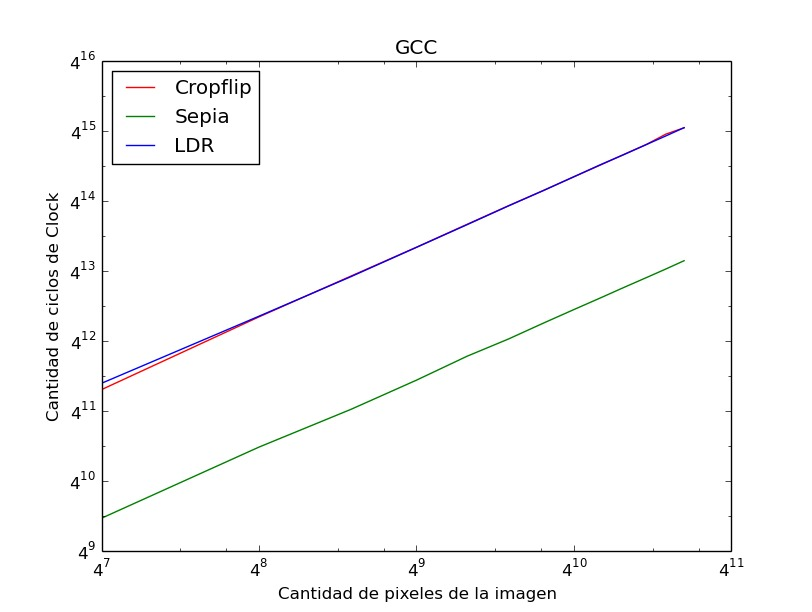
\includegraphics[scale=.50]{./imagenes/GCCO0.jpg}   
      }
    \end{floatrow}
\end{figure}



Bueno, si alguien hubiera dicho que sepia iba a ser el filtro mas rapido, le
hubieramos dicho que estaba loco.

Aqui el grafico de Clang

\begin{figure}[H]
    \centering
    \begin{floatrow}
      \ffigbox[\FBwidth]{\caption{Filtros con Clang -O0}}{%
        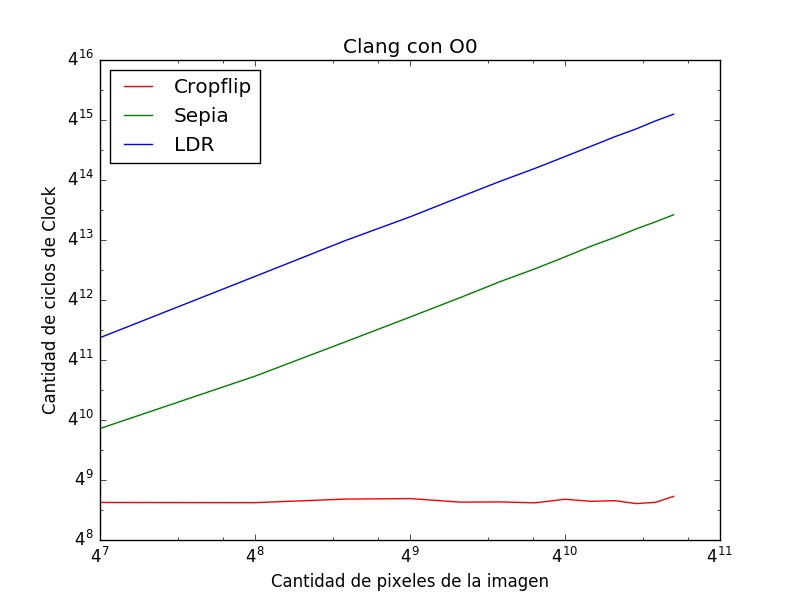
\includegraphics[scale=.50]{./imagenes/Clang0.jpg}   
      }
    \end{floatrow}
\end{figure}

Vemos que sin importar el filtro elegido, GCC le gana a clang, donde mas se nota es en Sepia, mientras que en Cropflip y LDR la diferencia es poca.


Ahora, vamos a repetir el mismo experimento pero variando las flags, esta vez vamos a usar
-O3 -Wall -std=c99 -pedantic -m64

\begin{figure}[H]
    \centering
    \begin{floatrow}
      \ffigbox[\FBwidth]{\caption{Filtros con GCC -O0}}{%
        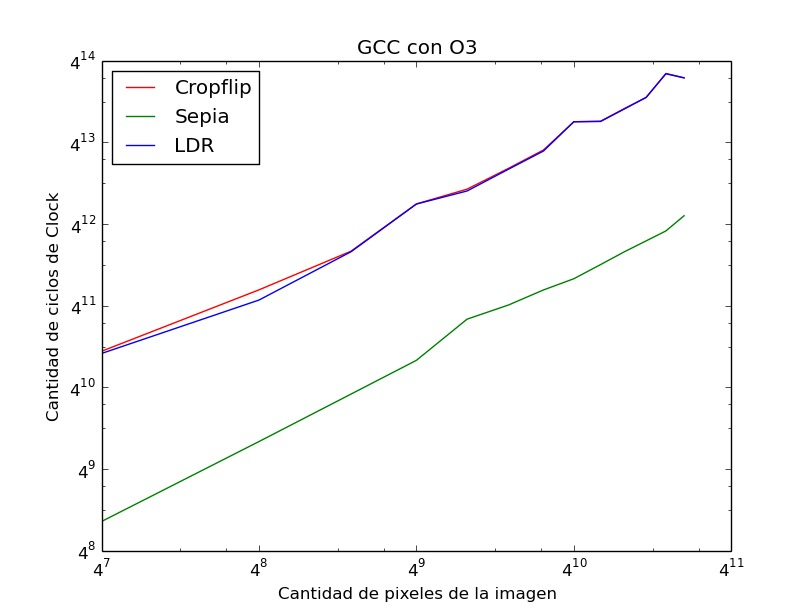
\includegraphics[scale=.50]{./imagenes/GCCO3.jpg}   
      }
    \end{floatrow}
\end{figure}


\begin{figure}[H]
    \centering
    \begin{floatrow}
      \ffigbox[\FBwidth]{\caption{Filtros con Clang -O0}}{%
        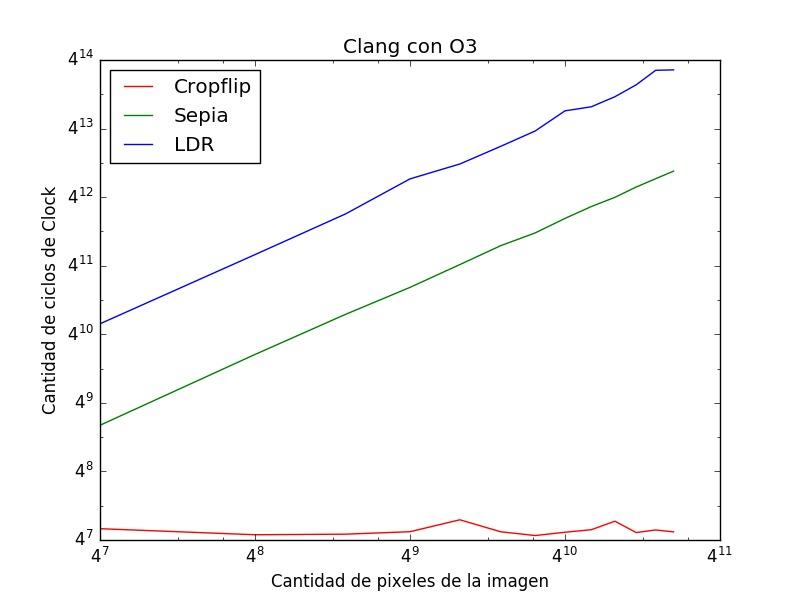
\includegraphics[scale=.50]{./imagenes/Clang3.jpg}   
      }
    \end{floatrow}
\end{figure}

Vemos que en Sepia gana GCC, en LDR gana Clang y en Cropflip hay empate tecnico


